\documentclass[reprint,english]{revtex4-1}

% language
\usepackage[utf8]{inputenc}
\usepackage[english]{babel}

% standard setup
\usepackage{physics,amssymb,array}
\usepackage{xcolor,graphicx,hyperref}
\usepackage{tikz,listings,multirow}
\usepackage{subfigure}
\usepackage{enumitem}

% hyperref coloring
\hypersetup{ %
  colorlinks,
  linkcolor={red!50!black},
  citecolor={blue!50!black},
  urlcolor={blue!80!black}}

% lstlisting coloring
\lstset{ %
  inputpath=,
  backgroundcolor=\color{white!88!black},
  basicstyle={\ttfamily\scriptsize},
  commentstyle=\color{magenta},
  language=C++,
  tabsize=2,
  stringstyle=\color{green!55!black},
  frame=single,
  keywordstyle=\color{blue},
  showstringspaces=false,
  columns=fullflexible,
  keepspaces=true}

% pretty matrix
\newcolumntype{C}[1]{>{\centering\arraybackslash$}p{#1}<{$}}

\begin{document}
% titlepage
\title{FYS3150 - Project 1 Report}
\author{Nils Johannes Mikkelsen}
\date{\today}
\noaffiliation
\begin{abstract}
Abstract.
\end{abstract}
\maketitle

% body
\section*{About Project 1}
This is a report for Project 1 in FYS3150 - Computational Physics at UiO, due September \(10^{\text{th}}\), 2018. The project description was accessed August \(27^{\text{th}}\), 2018 with this web address:\\
{\scriptsize\url{http://compphysics.github.io/ComputationalPhysics/doc/Projects/2018/Project1/pdf/Project1.pdf}}\\
All material written for this report can be found in this GitHub repository:\\
{\scriptsize\url{https://github.com/njmikkelsen/comphys2018}}
\section{Introduction}
It is the object of this report to investigate central finite difference approximation methods in relation to linear second order ordinary differential equations without first order terms. The report is most concerned with the accuracy of the approximation, including errors related to floating point arithmetic, and the efficiency of tridiagonal matrix equation algorithms used in the numerical integration. The algorithms presented in this report will finally be compared to standard matrix solving algorithms based on LU matrix decomposition.
\section{Theory}
\subsection{Linear Second Order Ordinary Differential Equations without First Order Terms}
\subsubsection{The general equation}
A linear second order ordinary differential equation (ODE) without first order terms can be written as
\begin{equation}\label{eq:main_differential_equation}
\dv[2]{x}y(x)+k(x)^2y(x)=f(x)
\end{equation}
where \(x\) and \(y=y(x)\) are the independent and dependent variables, \(k(x)\) is a variable coefficient and \(f(x)\) is the so-called \emph{source} term. The most famous example of equation \eqref{eq:main_differential_equation} in Physics is Newton's Second Law of Motion. Section \ref{sec:poisson_equation} introduces another common example, namely Poisson's equation from electrostatics.
\subsubsection{A specific case}\label{sec:specific_case}
Let \(k(x)=0\) and \(f(x)=-100e^{-10x}\) such that equation \ref{eq:main_differential_equation} may be simplified to
\begin{equation}\label{eq:specific_differential_equation}
\dv[2]{x}y(x)=-100e^{-10x}
\end{equation}
The solution to equation \eqref{eq:specific_differential_equation}, namely \(y(x)\), is easily found by integrating twice:
\begin{align}
\dv{x}y(x)&=-10^2\int\dd{x}e^{-10x}\nonumber\\
&=10e^{-10x}+C_1\nonumber\\[2mm]
y(x)&=10\int\dd{x}e^{-10x}+C_1x\nonumber\\
&=-e^{-10x}+C_1x+C_2\label{eq:general_solution_to_specific}
\end{align}
Furthermore, introducing the boundary conditions:
\[y(x=0)=y(x=1)=0\]
imposes restraints on \(C_1\) and \(C_2\) such that
\begin{equation}\label{eq:specific_solution_to_specific}
y(x)=1-(1-e^{-10})x-e^{-10x}
\end{equation}
\subsection{Poisson's Equation from Electrostatics}\label{sec:poisson_equation}
\subsubsection{Derivation}
Using Gaussian units, Gauss's law of electricity and the Maxwell-Faraday equation may be written as
\begin{align}
\div\vb{E}&=4\pi\rho\label{eq:gauss_law}\\
\curl\vb{E}&=-c^{-1}\pdv{t}\vb{B}\label{eq:maxwell-farady_equation}
\end{align}
where \(\vb{E}\) and \(\vb{B}\) are the electric field and the magnetic flux density, \(\rho\) is the scalar electric charge distribution and \(c\) is the speed of light.

Assuming electrostatics implies that \(\pdv*{\vb{B}}{t}=0\), which further implies that \(\curl\vb{E}=0\). As the curl of \(\vb{E}\) is zero, \(\vb{E}\) is defined by scalar electric potential \(\varphi\):
\begin{equation}\label{eq:electric_field_from_potential}
\vb{E}=-\grad\varphi
\end{equation}
Finally, combining equations \eqref{eq:gauss_law} and \eqref{eq:electric_field_from_potential} yields Poisson's equation:
\begin{equation}\label{eq:poisson_equation_electrostatics}
\laplacian\varphi=-4\pi\rho
\end{equation}
\newpage
\subsubsection{Further development using a spherical distribution}
Assuming a spherically symmetric charge distribution \(\rho=\rho(r)\) allows for further simplification of equation \eqref{eq:poisson_equation_electrostatics} (the angular terms in \(\laplacian\varphi\) are ignored due to symmetry):
\begin{align*}
\laplacian\varphi(r)&=r^{-2}\dv{r}\Big[r^2\dv{r}\varphi(r)\Big]=r^{-2}\Big[2r\varphi(r)+r^2\dv[2]{r}\varphi(r)\Big]\\
&=r^{-1}\Big[\varphi(r)+r\dv{r}\varphi(r)\Big]=r^{-1}\dv[2]{r}\Big[r\varphi(r)\Big]
\end{align*}
Finally, define \(\phi=\varphi(r)/r\) such that Poisson's equation can be written as
\begin{equation}\label{eq:final_poisson_equation}
\dv[2]{r}\phi(r)=-4\pi r\rho(r)
\end{equation}
Equation \eqref{eq:final_poisson_equation} is recognised as a special case of equation \eqref{eq:main_differential_equation} with
\[y(x)=\phi(x)\qcomma k(x)=0\qand f(x)=-4\pi x\rho(x)\]
To arrive on the specific case introduced in section \ref{sec:specific_case}, the charge distribution must be given by:
\[\rho(r)=\frac{25}{\pi}r^{-1}e^{-10r}\]
\subsection{Finite Difference Approximation Methods for Second Order Derivatives}\label{sec:finite_difference_methods}
The Taylor expansion of any single-variable function \(f(x)\), centered about \(x=a\), can be written as
\begin{align}
f(x)&= f(a)+f'(a)(x-a)+\frac{f''(a)}{2}(x-a)^2\nonumber\\
&\quad +\frac{f'''(a)}{6}(x-a)^3+\frac{f^{(4)}(a)}{24}(x-a)^4+\cdots\label{eq:second_order_taylor_expansion}
\end{align}

Let \(a=x_0\) and \(x=x_0\pm\Delta x\) such that:
\begin{align}
f(x_0\pm\Delta x)&=f(x_0)\pm f'(x_0)\Delta x+\frac{f''(x_0)}{2}{\Delta x}^2\nonumber\\
&\quad \pm\frac{f'''(x_0)}{6}{\Delta x}^3+\frac{f^{(4)}(x_0)}{24}{\Delta x}^4+\cdots
\end{align}
This implies that:
\begin{align*}
&f(x_0+\Delta x)+f(x_0-\Delta x)=\\
&2f(x_0)+f''(x_0){\Delta x}^2+\frac{f^{(4)}(x_0)}{12}{\Delta x}^4+\cdots
\end{align*}
Solving for \(f''(x_0)\) yields the central second order finite difference approximation for second order derivatives:
\begin{align}
f''(x_0)&=\frac{f(x_0-\Delta x)-2f(x_0)+f(x_0+\Delta x)}{{\Delta x}^2}\nonumber\\
&\quad -\frac{f^{(4)}(x_0)}{12}{\Delta x}^2-\cdots\label{eq:second_order_finite_difference_approximation}
\end{align}
\section{Method}
The main equation that is solved in this report is equation \eqref{eq:specific_differential_equation} with Dirichlet boundary conditions \(y(0)=y(1)=0\), such that the analytic solution is given by equation \eqref{eq:specific_solution_to_specific}. To limit the scope of the numerical solution, \(x\) values outside the range \([0,1]\) are ignored.
\subsection{Discretisation of The Differential Equation}\label{sec:discretise_diffeq}
To begin the process, the \(x\)-range \([0,1]\) is divided into \(n+1\) equal slices such that the continuous \(x\) axis is replaced by an \(x\) grid with \(n+2\) points. Each grid point is denoted by \(x_i\), where \(i\in\{0,1,\ldots,n+1\}\), and is seperated by a grid spacing of \(h=(x_{n+1}-x_0)/(n+1)\). As expected, the grid boundaries are \(x_0=0\) and \(x_{n+1}=1\), which implies that \(h=1/(n+1)\).

Furthermore, the continuous functions \(y(x)\) and \(f(x)\) are replaced by the discrete sets \(\{y_i\}\) and \(\{f_i\}\) respectively. The set elements are defined by \(y_i=y(x_i)\) and \(f_i=f(x_i)\). The Dirichlet boundary conditions demand that \(y_0=y_{n+1}=0\).

Using the discretised variables, equation \eqref{eq:specific_differential_equation} may be discretised using the finite difference approximation of second order derivatives from section \ref{sec:finite_difference_methods}:
\begin{equation}
y''(x_i)=\frac{y_{i-1}-2y_i+y_{i+1}}{h^2}+\order{h^2}
\end{equation}
where \(\order{h^2}\) is local truncation error. With \(n\) approximations, the global truncation error is \(n\order{h^2}\approx\order{h}\) for small \(h\). The differential equation may thus be written as a coupled system of linear equations:
\begin{align*}
y_0-2y_1+y_2&=h^2f_1\\
y_1-2y_2+y_3&=h^2f_2\\
\vdots&\\
y_{n-1}-2y_n+y_{n+1}&=h^2f_n
\end{align*}
As \(y_0=y_{n+1}=0\), this system may be written as a matrix equation:
\[\mqty[-2 & 1 & 0 & \cdots & \cdots & 0 \\
1 & -2 & 1 & 0 & \cdots & \vdots \\
0 & 1 & -2 & 1 & \cdots & \vdots \\
\vdots & 0 & 1 & \ddots & \ddots & 0 \\
\vdots & \vdots & \vdots & \ddots & -2 & 1 \\
0 & \cdots & \cdots & 0 & 1 & -2]\mqty[y_1\\y_2\\\vdots\\y_{n-1}\\y_n]
=h^2\mqty[f_1\\f_2\\\vdots\\f_{n-1}\\f_n]\]
By introducing the new variable \(\tilde{y}_i=y_i/h^2\), the matrix equation may be written as
\begin{equation}\label{eq:matrix_equation_to_solve}
D\tilde{\vb{y}}=\vb{f}
\end{equation}
where \(D\) is the left hand side tridiagonal matrix, and \(\tilde{\vb{y}}\) and \(\vb{f}\) are column vectors.
\newpage
\subsection{Matrix Equation Algorithms}
The goal now is to develope a series of algorithms that are capable of solving equation \eqref{eq:matrix_equation_to_solve}. The algorithms have varying ``degrees of knowledge" of the equation in that they are based on different assumptions. However, all algorithms assume the matrix is a square matrix. Limited by their assumptions, the scope of the algorithms' areas of application differ (although they obviously share the ability to solve equation \eqref{eq:matrix_equation_to_solve}) and thus solve the same matrix equations with different efficiencies.

Each algorithm is only focused on equation \eqref{eq:matrix_equation_to_solve}, thus the final solution \(\vb{y}\) requires an additional calculation. It involves calculating \(h^2\) and computing each element \(y_i=(h^2)\tilde{y}_i\), which in total amounts to \(n+1\) additional FLOPS for each algorithm.

To avoid having to reintroduce notation, the following definitions will be used throughout. Any linear matrix equation may be written as
\begin{equation}\label{eq:general_linear_matrix_equation}
M\vb{v}=\vb{u}
\end{equation}
where \(M\) is an \(n\times n\) matrix with entries \(m_{ij}\), and \(\vb{v}\) and \(\vb{u}\) are \(n\)-dimensional vectors with entries \(v_i\) and \(u_i\) respectively. Note that \(i,j\in\{1,\ldots,n\}\).
\subsubsection{General matrix equation algorithm:\\LU Decomposition}
The first algorithm to be presented in this report is the well-known LU-Decomposition solution. The process is divided into two components: the LU-factorisation and solving the resulting matrix equations. As it happens, Project 1 does not require the report to include an in-depth description of LU-Decompositioning. The details surrounding the algorithm are therefore ignored. Nevertheless, the general principle behind the solution is explained below. When later performing the LU-decomposition numerically, a standard algorithm supplied by the \emph{armadillo} library is used.

Suppose the matrix \(M\) may be written as the product of two matrices \(L\) and \(U\): \(M=LU\), where \(L\) is a unit (diagonal entries equals 1) \emph{lower} triangular matrix and \(U\) is an \emph{upper} triangular matrix. Equation \eqref{eq:general_linear_matrix_equation} may thus be written as \(L(U\vb{v})=\vb{u}\), which can be further separated as two matrix equations:
\begin{equation}\label{eq:LU_decomposed_equations}
U\vb{v}=\vb{y}\qand L\vb{y}=\vb{u}
\end{equation}
There are several algorithms for finding \(L\) and \(U\). Although not necessarily the most efficient, the one presented here is a simple algorithm:
\begin{enumerate}
\item \(M\) is row-reduced to echelon form \(U\) by a sequence of row-replacement operations (if possible).
\item Then, the same sequence of row-replacement operations reduces \(L\) to \(I\) (the identity matrix).
\end{enumerate}
\newpage
\noindent Having found \(L\) and \(U\), the next steps are as follows:
\begin{enumerate}
\item \(\vb{y}\) may be found by solving \(L\vb{y}=\vb{u}\), which is very simplified by the fact that \(L\) is unit lower triangular: Starting from the upper row, each element below the current diagonal entry is directly removed by simple row-operations.
\item Finally, the solution \(\vb{v}\) is found by solving \(U\vb{v}=\vb{y}\). The entries in \(\vb{v}\) may computed sequentially by a backward substitution, starting from the lowest row.
\end{enumerate}
The benefits of LU-Decompositioning really arises when solving several matrix equations on the form \(M\vb{v}=\vb{d}\), where \(\vb{d}\) may differ with each equation. Nontheless, the process is fairly quick in on itself: as opposed to Gaussian elimination's \(\order{n^3}\) FLOPS, LU-Decompositioning requires \(\order{2n^2}\) FLOPS (this includes both the LU-fatorisation and the solving of equations \eqref{eq:LU_decomposed_equations}).
\subsubsection{A generalised tridiagonal matrix equation algorithm}\label{sec:general_tridiagonal_algorithm}
The next matrix algorithm solves a tridiagonal matrix equation with arbitrary diagonal entries. The algorithm presented here is often known as the Thomas algorithm and is in principle just Gaussian elimination, however specialised for tridiagonal matrices.

As \(M\) is tridiagonal, Equation \eqref{eq:matrix_equation_to_solve} may be written as:
\[\mqty[b_1 & c_1 & 0 & \cdots & \cdots & 0 \\
a_1 & b_2 & c_2 & 0 & \cdots & \vdots \\
0 & a_2 & b_3 & c_3 & \cdots & \vdots \\
\vdots & 0 & a_3 & \ddots & \ddots & 0 \\
\vdots & \vdots & \vdots & \ddots & b_{n-1} & c_{n-1} \\
0 & \cdots & \cdots & 0 & a_{n-1} & b_n]\mqty[v_1 \\ v_2 \\ \vdots \\ v_{n-1} \\ v_n]=\mqty[u_1 \\ u_2 \\ \vdots \\ u_{n-1} \\ u_n]\]
such that the linear equations may be written as
\begin{align*}
b_1v_1+c_1v_2&=u_1\\
a_{i-1}v_{i-1}+b_iv_i+c_iv_{i+1}&=u_i\qc i=2,\ldots,n-1\\
a_{n-1}v_{n-1}+b_nv_n&=u_n
\end{align*}

The first step is to perform a so-called ``forward sweep" in which the lower diagonal is removed and the central diagonal is normalised:
\begin{enumerate}
\item The first equation is divided by \(b_1\) so that \(m_{11}=1\).
\item For each equation from \(i=2\) to \(i=n\):
\begin{enumerate}
	\item The current equation is normalised so that \(m_{i,i-1}=1\).
	\item The previous equation is subtracted from the current equation so that \(m_{i,i-1}=0\).
	\item The current equation is renormalised so that \(m_{ii}=1\).
\end{enumerate}
\end{enumerate}
\newpage
\noindent Having completed the forward sweep, the matrix equation now reads
\[\mqty[1 & \tilde{c}_1 & 0 & \cdots & \cdots & 0 \\
0 & 1 & \tilde{c}_2 & 0 & \cdots & \vdots \\
0 & 0 & 1 & \tilde{c}_3 & \cdots & \vdots \\
\vdots & 0 & 0 & \ddots & \ddots & 0 \\
\vdots & \vdots & \vdots & \ddots & 1 & \tilde{c}_{n-1} \\
0 & \cdots & \cdots & 0 & 0 & 1]\mqty[v_1 \\ v_2 \\ \vdots \\ v_{n-1} \\ v_n]=\mqty[\tilde{u}_1 \\ \tilde{u}_2 \\ \vdots \\ \tilde{u}_{n-1} \\ \tilde{u}_n]\]
where
\begin{align}
\tilde{c}_i&=\frac{c_i}{b_i-a_i\tilde{c}_{i-1}}\qq{with}\tilde{c}_1=\frac{c_1}{b_1}\\
\tilde{u}_i&=\frac{u_i-a_i\tilde{u}_{i-1}}{b_i-a_i\tilde{c}_{i-1}}\qq{with}\tilde{u}_1=\frac{u_1}{b_1}
\end{align}
A forward sweep thus consists of computing:
\begin{itemize}
\renewcommand\labelitemi{\(\times\)}
\renewcommand\labelitemii{\(\to\)}
\item \(\tilde{c}_1\) and \(\tilde{u}_1\). 2 FLOPS
\item For \(i=2,\ldots,n-1\): (\(n-2\) iterations)
	\begin{itemize}
	\item \(\alpha_i=b_i-a_i\tilde{c}_{i-1}\). 2 FLOPS
	\item \(\tilde{c}_i=c_i/\alpha_i\). 1 FLOPS
	\item \(\tilde{u}_i=(u_i-a\tilde{u}_{i-1})/\alpha_i\). 3 FLOPS
	\end{itemize}
\item \(\tilde{u}_n=(u_n-a_n\tilde{u}_{n-1})/(b_n-a_n\tilde{c}_{n-1})\). 5 FLOPS
\end{itemize}
The total number of FLOPS during a forward sweep is therefore
\begin{align}
\text{FLOPS}_{\text{sweep}}&=2+(n-2)(2+1+3)+5\nonumber\\
&=6n-5
\end{align}
Following the forward sweep, the solution \(\vb{v}\) is obtained via a backward substitution:
\begin{enumerate}
\item The final element is found directly: \(v_n=\tilde{u}_n\).
\item For each equation from \(j=n-1\) to \(j=1\):
\begin{enumerate}
	\item The previous equation is multiplied with \(\tilde{c}_j\) and subtracted from the current equation so that \(m_{j-1,j}=0\).
\end{enumerate}
\end{enumerate}
By the end of the substitution, the matrix \(M\) will have been row-reduced to the identity matrix and the coefficients of \(\vb{v}\) are determined using the recursive relation:
\begin{equation}
v_n=\tilde{u}_n\qc v_j=\tilde{u}_j-\tilde{c}_jv_{j+1}
\end{equation}
Calculating \(v_n\) requires 0 FLOPS, but calculating \(v_j\) requires 2 FLOPS. Thus in total:
\begin{equation}
\text{FLOPS}_{\text{sub}}=2(n-1)=2n-2
\end{equation}
which implies that the complete algorithm for solving any tridiagonal matrix equation requires
\begin{equation}
\text{FLOPS}_{\text{general}}=8n-7
\end{equation}
\subsubsection{A specialised tridiagonal matrix equation algorithm}\label{sec:special_tridiagonal_algorithm}
Having presented a generalised algorithm for solving tridiagonal matrix equations, this subsection will focus on a specialised algorithm that assumes each individual diagonal contains identical entries. Mathematically, this implies that
\[a_i=a\qc b_i=b\qand c_i=c,\]
which simplifies the linear equations to
\begin{align*}
bv_1+cv_2&=u_1\\
av_{i-1}+bv_i+cv_{i+1}&=u_i\qc i=2,\ldots,n-1\\
av_{n-1}+bv_n&=u_n
\end{align*}
The specialised algorithm is based on a simplification of \(\tilde{c}_i\) and \(\tilde{u}_i\) from the generalised algorithm:
\begin{align*}
\tilde{c}_i&=\frac{c_i}{b_i-a_i\tilde{c}_{i-1}}=\frac{\frac{c}{a}}{\frac{b}{a}-\tilde{c}_{i-1}}\\
\tilde{u}_i&=\frac{u_i-a_i\tilde{u}_{i-1}}{b_i-a_i\tilde{c}_{i-1}}=\frac{\frac{u_i}{a}-\tilde{u}_{i-1}}{\frac{b}{a}-\tilde{c}_{i-1}}
\end{align*}
The first step is to divide the first equation by \(b\) and all other equations by \(a\) such that the linear equations read
\begin{align*}
v_1+\rho_1v_2&=u'_1\\
v_{i-1}+\rho_2v_i+\rho_3v_{i+1}&=u'_i\qc i=2,\ldots,n-1\\
v_{n-1}+\rho_2v_n&=u'_n
\end{align*}
where
\begin{align*}
&\rho_1=\frac{c}{b}\qc\rho_2=\frac{b}{a}\qc\rho_3=\frac{c}{a},\\
&u'_1=\frac{u_1}{b}\qand u'_i=\frac{u_i}{a}\qq{for}i=2,\ldots,n.
\end{align*}
This initial operation requires 3 FLOPS for \(\rho_1\), \(\rho_2\) and \(\rho_3\), in addition to \(n\) FLOPS for \(\vb{u}'\). Hence,
\begin{equation}
\text{FLOPS}_{\text{setup}}=n+3
\end{equation}
Before even having started on the forward sweep, the tridiagonal matrix equation thus reads
\[\mqty[1 & \rho_1 & 0 & \cdots & \cdots & 0 \\
1 & \rho_2 & \rho_3 & 0 & \cdots & \vdots \\
0 & 1 & \rho_2 & \rho_3 & \cdots & \vdots \\
\vdots & 0 & 1 & \ddots & \ddots & 0 \\
\vdots & \vdots & \vdots & \ddots & \rho_2 & \rho_3 \\
0 & \cdots & \cdots & 0 & 1 & \rho_2]\mqty[v_1 \\ v_2 \\ \vdots \\ v_{n-1} \\ v_n]=\mqty[u'_1 \\ u'_2 \\ \vdots \\ u'_{n-1} \\ u'_n]\]
\newpage
The next step is to perform a simpler, although conceptually identical, forward sweep:
\begin{enumerate}
\item[] For each equation from \(i=2\) to \(i=n\):
\begin{enumerate}
	\item The previous equation is subtracted from the current equation so that \(m_{i,i-1}=0\).
	\item The current equation is renormalised so that \(m_{ii}=1\).
\end{enumerate}
\end{enumerate}
Having completed the forward sweep, the matrix equation now reads
\[\mqty[1 & \tilde{c}_1 & 0 & \cdots & \cdots & 0 \\
0 & 1 & \tilde{c}_2 & 0 & \cdots & \vdots \\
0 & 0 & 1 & \tilde{c}_3 & \cdots & \vdots \\
\vdots & 0 & 0 & \ddots & \ddots & 0 \\
\vdots & \vdots & \vdots & \ddots & 1 & \tilde{c}_{n-1} \\
0 & \cdots & \cdots & 0 & 0 & 1]\mqty[v_1 \\ v_2 \\ \vdots \\ v_{n-1} \\ v_n]=\mqty[\tilde{u}_1 \\ \tilde{u}_2 \\ \vdots \\ \tilde{u}_{n-1} \\ \tilde{u}_n]\]
where the new coefficients are
\begin{align}
\tilde{c}_i&=\frac{\rho_3}{\rho_2-\tilde{c}_{i-1}}\qq{with}\tilde{c}_1=\rho_1\\
\tilde{u}_i&=\frac{u'_i-\tilde{u}_{i-1}}{\rho_2-\tilde{c}_{i-1}}\qq{with}\tilde{u}_1=u'_1
\end{align}
\noindent The specialised forward sweep consists of computing:
\begin{itemize}
\renewcommand\labelitemi{\(\times\)}
\renewcommand\labelitemii{\(\to\)}
\item For \(i=2,\ldots,n-1\): (\(n-2\) iterations)
	\begin{itemize}
	\item \(\alpha_i=\rho_2-\tilde{c}_{i-1}\). 1 FLOPS
	\item \(\tilde{c}_i=\rho_3/\alpha_i\). 1 FLOPS
	\item \(\tilde{u}_i=(u'_i-\tilde{u}_{i-1})/\alpha_i\). 2 FLOPS
	\end{itemize}
\item \(\tilde{u}_n=(u'_n-\tilde{u}_{n-1})/(\rho_2-\tilde{c}_{n-1})\). 3 FLOPS
\end{itemize}
The total number of FLOPS during a specialised forward sweep is therefore
\begin{align}
\text{FLOPS}_{\text{special sweep}}&=(n-2)(1+1+2)+3\nonumber\\
&=4n-5
\end{align}

The backward substitution in the specialised algorithm is identical to the backward substitution in the generalised algorithm and will thus not be discussed here. The complete specialised algorithm therefore requires
\begin{equation}
\text{FLOPS}_{\text{special}}=7n-4
\end{equation}
This suggests that the specialised algorithm is about \(8/7\approx1.14\) times faster than the generalised algorithm.
\newpage
\subsubsection{A taylored matrix equation algorithm}
The fourth and final algorithm presented here is an algorithm taylored to the actual problem at hand, namely equation \eqref{eq:matrix_equation_to_solve}. The notation used here will match the original notation used in section \ref{sec:discretise_diffeq}, note in particular:
\[M=D\qc\vb{v}=\vb{y}\qand\vb{u}=h^2\vb{f}\]
Furthermore, the diagonal entries are as follows:
\[a=c=1\qand b=-2\]
In order to avoid having to multiply by \(h^2\), the equation is written in terms of \(\tilde{y}_i=y_i/h^2\). Moreover, when the first equation is divided by \(-2\) and the rest are kept the same, the linear system of equations read
\begin{align*}
\tilde{y}_1-\frac{1}{2}\tilde{y}_2&=-\frac{1}{2}f_1\\
\tilde{y}_{i-1}-2y_i+\tilde{y}_{i+1}&=f_i\qc i=2,\ldots,n-1\\
\tilde{y}_{n-1}-2\tilde{y}_n&=f_n
\end{align*}
which in matrix form is:
\[\mqty[1 & -\frac{1}{2} & 0 & \cdots & \cdots & 0 \\
1 & -2 & 1 & 0 & \cdots & \vdots \\
0 & 1 & -2 & 1 & \cdots & \vdots \\
\vdots & 0 & 1 & \ddots & \ddots & 0 \\
\vdots & \vdots & \vdots & \ddots & -2 & 1 \\
0 & \cdots & \cdots & 0 & 1 & -2]\mqty[\tilde{y}_1 \\ \tilde{y}_2 \\ \vdots \\ \tilde{y}_{n-1} \\ \tilde{y}_n]=\mqty[-\frac{1}{2}f_1 \\ f_2 \\ \vdots \\ f_{n-1} \\ f_n]\]

%By performing a forward sweep in the same manner as presented in the specialised matrix equation algorithm, the resulting matrix equation is
\[\mqty[1 & -\frac{1}{2} & 0 & \cdots & \cdots & 0 \\
0 & 1 & \tilde{c}_2 & 0 & \cdots & \vdots \\
0 & 0 & 1 & \tilde{c}_2 & \cdots & \vdots \\
\vdots & 0 & 1 & \ddots & \ddots & 0 \\
\vdots & \vdots & \vdots & \ddots & 1 & \tilde{c}_{n-1} \\
0 & \cdots & \cdots & 0 & 0 & 1]\mqty[\tilde{y}_1 \\ \tilde{y}_2 \\ \vdots \\ \tilde{y}_{n-1} \\ \tilde{y}_n]=\mqty[\tilde{f}_1 \\ \tilde{f}_2 \\ \vdots \\ \tilde{f}_{n-1} \\ \tilde{f}_n]\]
where
\begin{align}
\tilde{c}_i&=\frac{1}{-2-\tilde{c}_{i-1}}\qq{with}\tilde{c}_1=-\frac{1}{2}\\
\tilde{f}_i&=\frac{f_i-\tilde{f}_{i-1}}{-2-\tilde{c}_{i-1}}\qq{with}\tilde{f}_1=-\frac{1}{2}f_1
\end{align}
The relationship between \(\tilde{c}_i\) and \(\tilde{f}_i\) is immediately noticeable:
\begin{equation}\label{eq:f_tilde_recursion_relation}
\tilde{f}_i=(f_i-\tilde{f}_{i-1})\tilde{c}_i=(\tilde{f}_{i-1}-f_i)(-\tilde{c}_i)
\end{equation}
(The reasoning behind the second equality will become apparent in due time.)
\newpage
The next step is to explore \(\tilde{c}_i\) a little more in detail. For starters, it may be written as
\begin{equation}\label{eq:tilde_c_requirement}
\tilde{c}_i=\frac{-1}{2+\tilde{c}_{i-1}}\qq{with}\tilde{c}_1=-\frac{1}{2}
\end{equation}
The goal is to rewrite the expression on a closed form (without chained fractions). By writing out the first iterations, a clear pattern emerges:
\begin{align*}
\tilde{c}_2&=\frac{-1}{2-\frac{1}{2}}=-\frac{2}{3}\\
\tilde{c}_3&=\frac{-1}{2-\frac{2}{3}}=-\frac{3}{4}\\
\tilde{c}_4&=\frac{-1}{2-\frac{3}{4}}=-\frac{4}{5}
\end{align*}
It is apparent that \(\tilde{c}_i\) behaves according to \(-i/(i+1)\). However, in order for \(\tilde{c}_i=-i/(i+1)\), equation \eqref{eq:tilde_c_requirement} must be satisfied:
\[\frac{-1}{2+\tilde{c}_{i-1}}=\frac{-1}{2+\big(\frac{i-1}{i}\big)}=\frac{-i}{2i-i+1}=-\frac{i}{i+1}=\tilde{c}_i\]
Hence, \(\tilde{c}_i=-i/(i+1)\), which implies that to calculate \eqref{eq:f_tilde_recursion_relation} requires only 2 FLOPS for \((-\tilde{c}_i)\) and 2 additional FLOPS for \(\tilde{f}_i\). Both \((-\tilde{c}_i)\) and \(\tilde{f}_i\) require \(n\) iterations such that the taylored forward sweep requires
\begin{align}
\text{FLOPS}_{\text{taylored sweep}}&=n(2+2)+1\nonumber\\
&=4n+1
\end{align}
(The \(+1\) stems from the computation of \(\tilde{f}_1\).)

Having calculated \((-\tilde{c}_i)\) and \(\tilde{f}_i\), the backward substitution is completed using the following recursion relation (the concept has already been explained in previous algorithms):
\begin{equation}
\tilde{y}_n=\tilde{f}_n\qand\tilde{y}_j=\tilde{f}_j+(-\tilde{c}_j)\tilde{y}_{j+1}
\end{equation}
The number of FLOPS required for the taylored substitution is the same as in previous algorithms. In total, the number of FLOPS for completing the taylored algorithm is
\begin{equation}
\text{FLOPS}_{\text{taylored}}=6n-1
\end{equation}
This suggests that the taylored algorithm is about \(8/6\approx1.34\) times faster than the generalised algorithm, and about \(7/6\approx1.17\) times faster than the specialised algorithm. It is likely that the actual efficiency of the taylored algorithm is even greater than this due to its ability to vectorise some of its calculations (in particular \((-\tilde{c}_i)\)). Among the algorithms presented in this report, the ability to vectorise some computations is unique to the taylored approach, and often may improve the accuracy significantly.
\newpage
\subsection{Comparing The Numerical Solutions}
\subsubsection{Accuracy}
Seeing that the differential equation (eq.\eqref{eq:specific_differential_equation}) was solved analytically in section \ref{sec:specific_case}, this provides an excellent opportunity to compare the numerical solutions to the exact solution.

The relative error between the numerial and exact solution in \(x_i\) is given by
\begin{equation}\label{eq:relative_error}
\epsilon_i=\left|\frac{y(x_i)-y_i}{y(x_i)}\right|
\end{equation}
The relative error is highly dependent on the value of \(n\), often changing by orders of magnitude. Thus instead of the regular relative error, this report will study the magnitude of the relative error with respect to the magnitude of \(h\) (i.e., \(\log(h)\)):
\begin{equation}\label{eq:relative_error_magnitude}
\varepsilon_i=\log(|\epsilon_i|)=\log\bigg[\left|\frac{y(x_i)-y_i}{y_i}\right|\bigg]
\end{equation}
(Here, it is implied that the logarithm is with respect to base 10.)
The greater number of FLOPS an algorithm requires, the more prone the algorithm is to accumulated errors from floating point arithmetic. This error is also contained in \(\epsilon_i\), thus the various algorithms may achieve different relative errors depending on the number of grid points.
\subsubsection{Efficiency}
As already mentioned, the different algorithms require different number of FLOPS, thus performing with different efficiencies. Measuring the efficiency of an algorithm is easily done using the computer's CPU time. However, the uncertainty in this calculation depends on the CPU time granularity, and the precision of the time ticks. The granularity is easily found, but the precision of the ticks is difficult to handle. Thus, the uncertainty should be considered as an estimate of the standard deviation as opposed to a strict uncertainty.
\clearpage
\section{Results}
\subsection{The generalised algorithm}
Figures \ref{fig:gen_alg_n10}, \ref{fig:gen_alg_n100} and \ref{fig:gen_alg_n1000} show plots of the numerical solutions provided by the generalised algorithm with \(n=10\), 100 and 1000 grid points respectively. It is immediately obvious that this algorithm quickly approaches the exact solution: already with \(n=100\), the difference is minimal. Furthermore, table \ref{tab:time_gen_alg_n10} shows the average time spent during calculation. The impact from increasing \(n\) from 10 to 100 is actually much less (in proportion) to increasing \(n\) from 10 to 100. That is, there seems to be a non-linear relationship between \(n\) and time spent.
\begin{figure}[h]
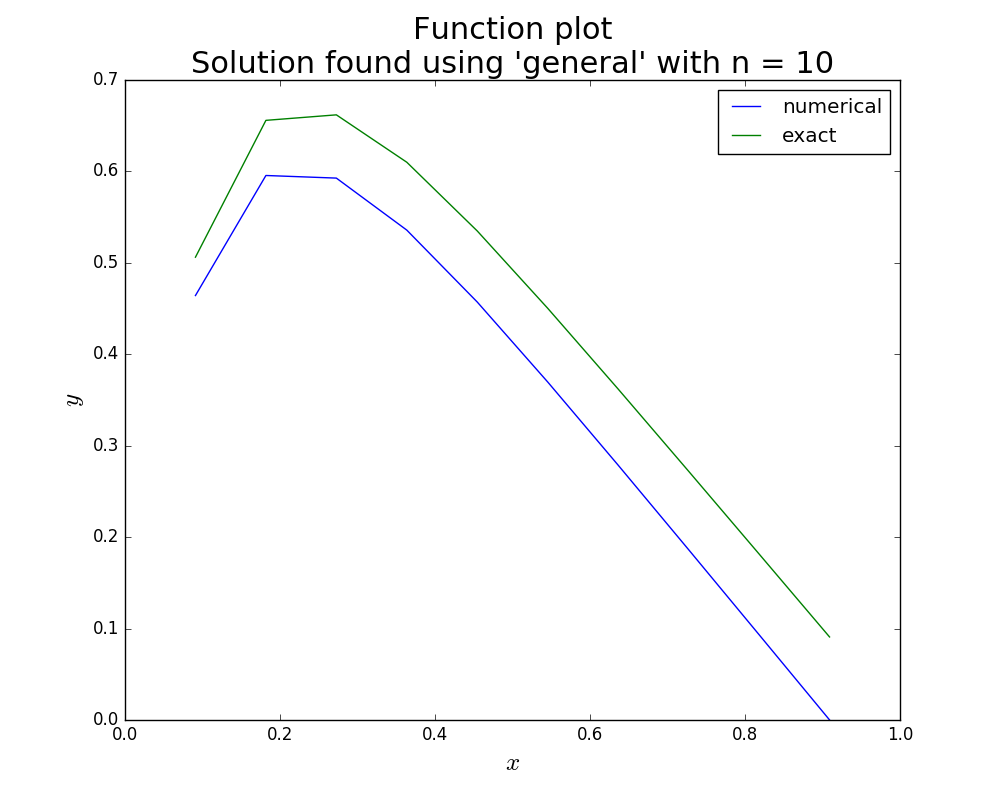
\includegraphics[scale=0.28]{figures/general_10_funcplot.png}
\caption{A plot of the numerical solution on top of the exact solution. Numerical solution calculated using the generalised algorithm with \(n=10\).}\label{fig:gen_alg_n10}
\end{figure}
\begin{figure}[h]
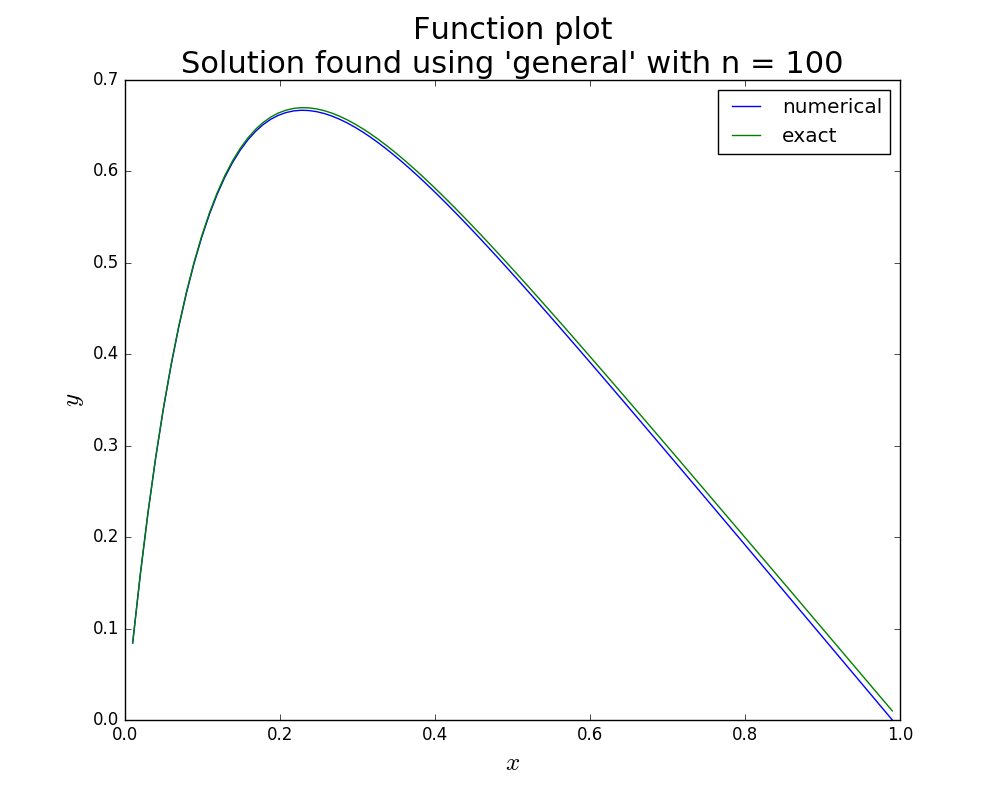
\includegraphics[scale=0.28]{figures/general_100_funcplot.png}
\caption{A plot of the numerical solution on top of the exact solution. Numerical solution calculated using the generalised algorithm with \(n=100\).}\label{fig:gen_alg_n100}
\end{figure}
\begin{figure}[h]
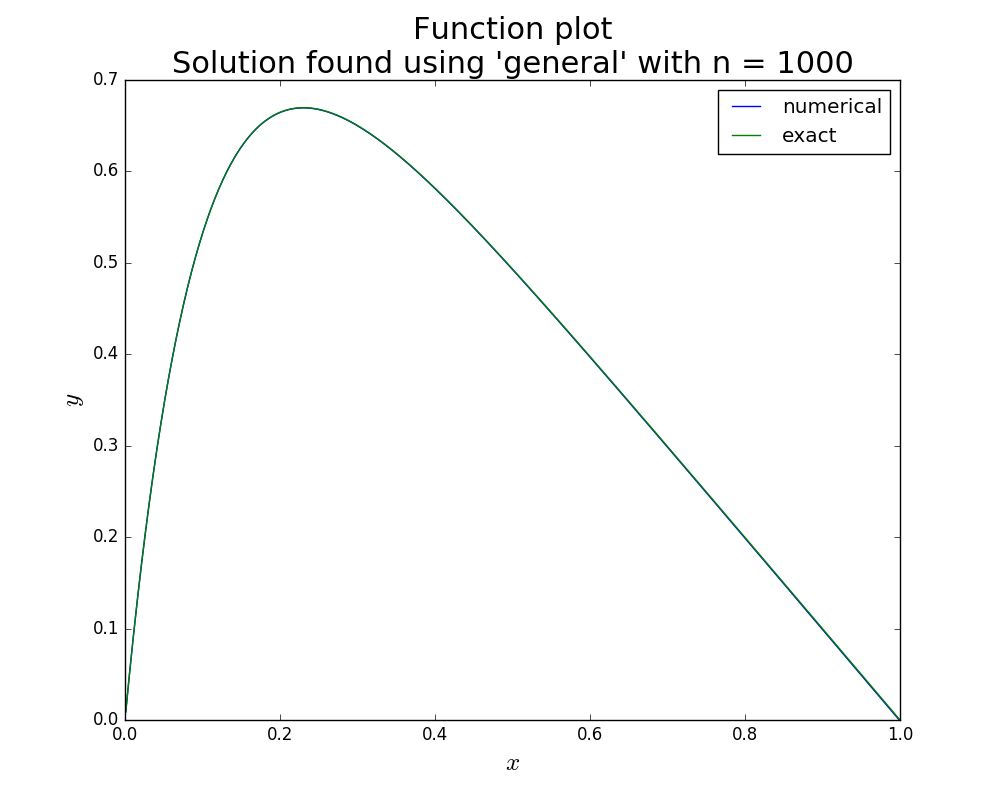
\includegraphics[scale=0.28]{figures/general_1000_funcplot.png}
\caption{A plot of the numerical solution on top of the exact solution. Numerical solution calculated using the generalised algorithm with \(n=1000\).}\label{fig:gen_alg_n1000}
\end{figure}
\begin{table}[h]
\caption{Average time spent by the generalised algorithm during a calculation.}\label{tab:time_gen_alg_n10}
\begin{tabular}{|c|c|}
\hline
\(n\) & time spent \\\hline
  10  & 0.010 ms \\\hline
 100  & 0.019 ms \\\hline
1000  & 0.126 ms \\\hline
\end{tabular}
\end{table}
\subsection{The specialised and taylored algorithms}


















\clearpage
\section{Discussion}
\section{Conclusion}
%\cite{dirac}\cite{einstein}
%\bibliographystyle{plain}
%\bibliography{references}
	 






\end{document}